\documentclass{article}

\usepackage{fontspec}
\usepackage{fullpage}
\usepackage{multicol}
\usepackage{multirow}
\usepackage{tikz}

\begin{document}

\newfontfamily\swfill{SuttonSignWritingFill.ttf}
\newfontfamily\swline{SuttonSignWritingLine.ttf}
\newcommand{\bul}{\hfil$\bullet$&}
\renewenvironment{glossary}{\begin{multicols}{5}\begin{center}}{\end{center}\end{multicols}}
\setcounter{secnumdepth}{0}
\setlength{\columnseprule}{1pt}

\section{Supplement For Lesson 2}

\begin{center}
\it
Objectives inspired by, vocabulary transcribed from, and sentences and stories by Bill Vicars.

Handshape photos by Adam Frost.

No endorsement implied nor given by either.
\end{center}

\subsection{Objectives}

\begin{tabular}{p{1cm}p{14cm}}
\bul I have completed the objectives for this lesson.\\
\bul I am able to read each letter of the fingerspelled alphabet.\\
\bul I am able to read the numbers 6--10.\\
\bul I am able to list the seven categories of SignWrititng in order.\\
\bul I am able demonstrate the meaning and form of the symbol groups in the hand category in order.\\
\bul I understand which type of handshapes are in Symbol Groups one, two, and three.\\
\bul I know what palmshape means.\\
\bul I am able to draw the fist palmshape in all forms.\\
\bul I am able to draw and demonstrate what fill one means.\\
\bul I am able to draw and demonstrate what rotation means.\\
\bul I am able to read, write, and sign the ASL handshapes in symbol group one.\\
\bul I am able to recognize the vocabulary for lesson.\\
\bul I am able to read the practice sentences for this lesson.\\
\bul I am able to read the practice stories for this lesson.\\
\end{tabular}

\subsection{The Fingerspelled Alphabet}

\begin{center}
\begin{tabular}{*{5}{c}}
\textbf{A}&\textbf{B}&\textbf{C}&\textbf{D}&\textbf{E}\\
B510x508S1f720490x493&B507x511S14720493x489&B509x510S16d20492x490&B508x515S10110492x485&B508x508S14a20493x493\\
\textbf{F}&\textbf{G}&\textbf{H}&\textbf{I}&\textbf{J}\\
B511x515S1ce20489x485&B515x508S1f000486x493&B515x508S11502485x493&B511x510S19220490x491&B519x519S19220498x500S2a20c481x482\\
\textbf{K}&\textbf{L}&\textbf{M}&\textbf{N}&\textbf{O}\\
B515x515S14020486x485&B512x515S1dc20488x485&B510x513S18d20490x488&B511x513S11920490x487&B508x508S17620492x492\\
\textbf{P}&\textbf{Q}&\textbf{R}&\textbf{S}&\textbf{T}\\
B516x512S14021485x488&B515x512S1f021485x489&B508x515S11a20493x485&B508x508S20320493x493&B508x510S1fb20493x491\\
&\textbf{U}&\textbf{V}&\textbf{W}\\
&B508x515S11520493x485&B508x515S10e20493x485&B509x515S18720491x486\\
&\textbf{X}&\textbf{Y}&\textbf{Z}\\
&B511x513S10620490x487&B514x510S19a20486x490&B519x518S10020481x488S2450a488x483\\
\end{tabular}
\end{center}

\subsection{The Numbers 6--10}

\begin{center}
\begin{tabular}{*{5}{c}}
\textbf{Six}&\textbf{Seven}&\textbf{Eight}&\textbf{Nine}&\textbf{Ten}\\
B509x515S18720491x486&B511x514S1a520490x486&B511x514S1bb20490x486&B511x515S1ce20489x485&B513x528S1f540488x504S2a538494x472\\
\end{tabular}
\end{center}

\subsection{SignWriting Categories}

Every SignWriting symbol has been assigned to one of seven categories, and each category has between one and ten Symbol Groups within it.
This is very similar to knowing whether a letter in English in a consonant or vowel, it's just that SignWriting has a larger vocabulary of groups of base symbols.

In order to be considered literate you will be able to know which categories each base symbol is in.
Because the base symbols of SignWriting are organized by category, if you can do the list of Symbol Groups in order then you can also list the categories in order but knowing the order of categories is much more likely to help with knowing the order of the base symbols.

\begin{center}
\begin{tabular}{ccc@{\hskip 2cm}ccc}
\textbf{Category}&\textbf{Example}&\textbf{Name}&\textbf{Category}&\textbf{Example}&\textbf{Name}\\
\textbf{1}&B508x515S10000493x485&Hand       &\textbf{2}&B507x508S22a00494x493&Movement\\
\textbf{3}&B506x504S2f700494x497&Timing     &\textbf{4}&B518x518S30a00482x483&Face    \\
\textbf{5}&B523x506S36e00477x494&Body       &\textbf{6}&B521x521S37f00480x480&Detail  \\
\textbf{7}&B537x504S38700463x496&Punctuation\\
\end{tabular}
\end{center}

You can't move on to the next lesson until you can say ``hand, movement, timing, face, body, detail, punctuation.

\subsection{The Hand Category}

The first category is called ``Hand'' and has ten symbol groups roughly based on the first ten numbers in ASL.
You will eventually be able to recite the informal names of all thirty symbol groups in order as easily as you can recite the alphabet.
The symbol groups can be thought of a three groups of ten, and the first ten are extremely easy to remember.

\begin{center}
\begin{tabular}{ccc@{\hskip 5mm}ccc}
\textbf{Symbol}&&&\textbf{Symbol}\\
\textbf{Group}&\textbf{Name}&\textbf{Example}&\textbf{Group}&\textbf{Name}&\textbf{Example}\\
\textbf{1}&One  &B508x515S10000493x485&\textbf{2} &Two  &B508x515S10e00493x485\\
\textbf{3}&Three&B512x515S11e00489x485&\textbf{4} &Four &B511x516S14400489x485\\
\textbf{5}&Five &B512x516S14c00489x485&\textbf{6} &Six  &B509x515S18600491x485\\
\textbf{7}&Seven&B510x515S1a400490x485&\textbf{8} &Eight&B510x515S1ba00490x485\\
\textbf{9}&Nine &B510x515S1cd00490x485&\textbf{10}&Thumb&B512x508S1f500488x493\\
\end{tabular}
\end{center}

It's important to remember that these names are informal.
B510x515S1cd00490x485 does not correspond to the ASL number nine though these unofficial names are reminiscent.
For instance compare B510x515S1cd00490x485 with B511x515S1ce20489x485.
You will learn the official names but for learning SignWriting, we are just asking you to know the informal names in order but not yet --- though it would be surprising to not remember them.

\subsection{The Symbol Groups One, Two, and Three}

The first Symbol Group we informally call one, though it's official name is ``Index''.
Symbol Group Index (One) consists of all handshapes where the index finger features prominently.
If there are other fingers, they are a group of fingers and secondary to the handshape.

The actual handshapes and their order will be covered a little later in this lesson.

The second Symbol Group we informally call two, though it's official name is ``Index Middle''.
Symbol Group Index Middle (Two) consists of all handshapes with the index and middle finger extended and no other fingers extended.

The actual handshapes and their order, as with the remaining symbol groups in category one, will be covered in future lessons.

The third Symbol Group we informally call three, though it's official name is ``Index Middle Thumb''.
Symbol Group Index Middle Thumb (Three) consists of all handshapes with the index, middle fingers, and thumb extended and no other fingers extended.

Before you can consider this lesson complete, you need to be able to list off the symbol groups as:
``one, two, three''.

That shouldn't be too hard for you.

\subsection{Palmshapes}

Each hand shape has a palmshape at its root, the shape you draw first before decorating it with fingers.
Each palmshape represents how tightly the ``missing'' fingers are held together.
They come in two primary types of fist and heel.

In the fist type are fist (meaning that the missing fingers are held tightly),
circle (meaning that the missing fingers are held loosely),
side (meaning that the fingers are open and held firm and not actually missing),
cup (meaning that the fingers are open and relaxed and not actually missing), and
flat (meaning that the hand is all the way open).

In the heel type are fist (meaning that the missing fingers are held tightly),
and flat (meaning that the hand is all the way open).

The heel palmshapes are technically redundant, but are important in correctly expressing meaning by (and to) someone who is fluent in ASL.
As an example: point your fingers straight forward, open your hand and pretend you are placing your palm on an imaginary table with your palm pointing straight down.
This can be either B512x516S14c50488x485 or B515x509S14d14485x491.
Both are correct recordings of this handshape and position, but (depending on the word and context) one will be the most correct.
If looking up an unfamiliar sign it may help to consider both options.

We will spend some time on each of these palmshapes, but here are examples of each so you know what you are looking at.

\begin{center}
\begin{tabular}{ccccc}
\textbf{Fist}     &B500x500S20300500x500&&\textbf{Circle}   &B500x500S17600500x500\\
\textbf{Side}     &B500x500S16800500x500&&\textbf{Cup}      &B500x500S17100500x500\\
\textbf{Flat}     &B500x500S15a00500x500\\
\textbf{Fist Heel}&B500x500S20410500x500&&\textbf{Flat Heel}&B500x500S15c10500x500\\
\end{tabular}
\end{center}

\subsection{The Fist Palmshape}

Yes, I am aware that we just talked about this but $\ldots$ the fist palmshape represents holding the hand tightly.

\begin{center}
\begin{tabular}{r*{6}{c}}
&\textbf{Fill 1}&\textbf{Fill 2}&\textbf{Fill 3}&\textbf{Fill 4}&\textbf{Fill 5}&\textbf{Fill 6}\\
\multirow{2}{*}{\textbf{Right Hand}}&
B500x500S20300500x500&
B500x500S20310500x500&
B500x500S20320500x500&
B500x500S20330500x500&
B500x500S20340500x500&
B500x500S20350500x500\\
&
\tikz{\draw[thick](0,0)rectangle(10pt,10pt);}&
\tikz{\draw[thick](0,0)rectangle(10pt,10pt);\draw[thick](5pt,10pt)--(5pt,0);\draw[thick](10pt,10pt)--(5pt,0);\draw[thick](5pt,10pt)--(10pt,0);}&
\tikz{\draw[thick](0,0)rectangle(10pt,10pt);\draw[thick](0,0)--(10pt,10pt);\draw[thick](0,10pt)--(10pt,0);}&
\tikz{\draw[thick](0,0)rectangle(10pt,10pt);\draw[thick](-3pt,7pt)--(13pt,7pt);}&
\tikz{\draw[thick](0,0)rectangle(10pt,10pt);\draw[thick](5pt,10pt)--(5pt,0);\draw[thick](10pt,10pt)--(5pt,0);\draw[thick](5pt,10pt)--(10pt,0);\draw[thick](-3pt,7pt)--(13pt,7pt);}&
\tikz{\draw[thick](0,0)rectangle(10pt,10pt);\draw[thick](0,0)--(10pt,10pt);\draw[thick](0,10pt)--(10pt,0);\draw[thick](-3pt,7pt)--(13pt,7pt);}\\
\multirow{2}{*}{\textbf{Left Hand}}&
B500x500S20308500x500&
B500x500S20318500x500&
B500x500S20328500x500&
B500x500S20338500x500&
B500x500S20348500x500&
B500x500S20358500x500\\
&
\tikz{\draw[thick](0,0)rectangle(10pt,10pt);}&
\tikz{\draw[thick](0,0)rectangle(10pt,10pt);\draw[thick](5pt,10pt)--(5pt,0);\draw[thick](0,10pt)--(5pt,0);\draw[thick](0,0)--(5pt,10pt);}&
\tikz{\draw[thick](0,0)rectangle(10pt,10pt);\draw[thick](0,0)--(10pt,10pt);\draw[thick](0,10pt)--(10pt,0);}&
\tikz{\draw[thick](0,0)rectangle(10pt,10pt);\draw[thick](-3pt,7pt)--(13pt,7pt);}&
\tikz{\draw[thick](0,0)rectangle(10pt,10pt);\draw[thick](5pt,10pt)--(5pt,0);\draw[thick](0,10pt)--(5pt,0);\draw[thick](0,0)--(5pt,10pt);\draw[thick](-3pt,7pt)--(13pt,7pt);}&
\tikz{\draw[thick](0,0)rectangle(10pt,10pt);\draw[thick](0,0)--(10pt,10pt);\draw[thick](0,10pt)--(10pt,0);\draw[thick](-3pt,7pt)--(13pt,7pt);}\\
\end{tabular}
\end{center}

The first row is what the right hand will look like in most of this manual.
The second row is an approximation of what it will look like when you write it.
The third row is what the left hand will look like in most of this manual.
The fourth row is an approximation of what it will look like when you write it.

Most of the lessons will not show you how to hand print the glyphs, and we don't have to because hand printing is as systematic as the rest of SignWriting.
Whenever you are trying to print a handshape, there are four phases: palmshape, palm fill, fingers, and floor fill.

For phase 1 we start with the palmshape:
are you drawing the square fist, the rectangle of a side or flat heel, or the half square of the fist heel;
the full circle or the partial circle of a cup;
or are you drawing the five sided flat?
And before you write it down, which rotation are you going to need?

For phase 2 we have three considerations:
for fills 1 and 4: move on to the next phase;
for fills 2 and 5: draw a line down the middle, and then draw an ``X'' through the correct half to indicate the shading;
for fills 3 and 6: draw an ``X'' in the palmshape to indicate full shading.

For phase 3 we decorate the edges with any fingers that may exist.
If the fingers extend outside of the palmshape, then that part is simple enough but pay attention to things like is it up or to the side, and which corner is it next to?
If the fingers push into the palmshape (like with number 4) then draw the finger crossing that side of the palmshape---with the finger being both in and sticking out a little.
If there aren't any fingers, like in these examples, then just move on to the final phase.

For phase 4 we have three considerations:
for fills 1--3, we are already done;
For fills 4--6 and handshapes without finger (or with only internal fingers) we draw a line through the top portion of the glyph which sticks out on both ends;
for fills 4--6 and handshapes with fingers, we draw a line through the fingers.

SignWriting has a cursive form which is aimed at ease and speed of writing and, just like with cursive in English, tends to be a personalized and assumes that you know enough of the language to ``fill in'' the extra pieces.
If you find yourself wanting to write just a bit faster, you can take a look at \texttt{https://www.signwriting.ord/lessons/cursive/handwriting/}.

\subsection{The First Fill}

\subsubsection{Hand Symbols}

\begin{center}
B508x515S10000493x485 B508x515S10e00493x485 B512x515S11e00489x485
\end{center}

Any symbol drawn in the first fill means that the signer's palm is facing the signer.
For all the hand symbols, the empty portion represents the signer's palm and the filled portion represents the back of the hand.
So for fill one, if the hand was open you would be able to see all of your palm and none of the back of your hand --- leaving fill one an empty symbol.

\subsubsection{Movement Symbols}

\begin{center}
B508x515S22b00492x485 B508x515S25600492x485 B508x515S26600492x485
\end{center}

Any symbol drawn in the first fill means that the right hand is doing the movement, so for all of these the right hand is doing the moving.

\subsubsection{Everything Else}

\begin{center}
B506x504S2f700494x497 B518x518S30a00482x483 B537x504S38700463x496
\end{center}

The fills for other categories tend to be a bit more variable.
Here we have fast, eyebrows up, and comma.

\subsection{Rotation}

In some cases, rotation does not provides semantic information so only one rotation exists:
B518x518S30a00482x483

For most symbols, rotation is simply one of eight directions:
B507x508S22a00494x493 B507x507S22a01494x493 B508x507S22a02493x494 B507x507S22a03494x493 B507x508S22a04494x493 B507x507S22a05494x493 B508x507S22a06493x494 B507x507S22a07494x493

And some symbols have mirroring:
B508x515S10000493x485 B511x515S10007490x485 B515x508S10006485x493 B515x511S10005485x490 B508x515S10004493x485 B511x515S10003490x485 B515x508S10002485x493 B515x511S10001485x490
B508x515S10008493x485 B511x515S10009490x485 B515x508S1000a485x493 B515x511S1000b485x490 B508x515S1000c493x485 B511x515S1000d490x485 B515x508S1000e485x493 B515x511S1000f485x490

For symbols that represent something parallel to the wall, the symbol represents the direction if you were holding the paper parallel to the wall in front of you.
For instance, {\small B508x515S10000493x485} means your index finger is pointing up while {\small B515x508S10002485x493} means that your index finger is pointing to your left.

For symbols that represent something parallel to the floor, the symbol represents the direction if you set the paper on the floor in front of you.
For instance, {\small B508x515S10030493x485} means your index finger is pointing forward, {\small B515x508S10032485x493} means that your index finger is pointing to your left, and {\small B508x515S10034493x485} means your index finger is pointing back toward yourself.

\subsection{ASL Handshapes From Symbol Group One}

The five handshapes in Symbol Group One used by ASL in order are:
{\em
Index;
Index on Circle;
Index on Angle;
Index Bent;
and Index Cup.
}

Before we introduce these handshapes, let's review how to write them.
First phase is palmshape in the correct rotation;
second phase is the base fill, possibly for the correct half of the palmshape;
third phase is fingers, which for most of these handshapes is one line on the correct corner for the fill, but for index on angle is three fingers on the correct corners for the fill;
fourth and final phase is the line for phases 4, 5, and 6.

For the first few of these we will be showing some examples of what the final form may look like, and we are confident that you can handle the rest on your own.

\subsubsection{The Index Handshape}

\begin{center}
\begin{tabular}{r*{6}{c}}
&\textbf{Fill 1}&\textbf{Fill 2}&\textbf{Fill 3}&\textbf{Fill 4}&\textbf{Fill 5}&\textbf{Fill 6}\\
\multirow{3}{*}{\textbf{Right Hand}}&
B508x515S10000493x485&
B508x515S10010493x485&
B508x515S10020493x485&
B508x515S10030493x485&
B508x515S10040493x485&
B508x515S10050493x485\\
&
\tikz{\draw[thick](0,0)rectangle(10pt,10pt);\draw[thick](10pt,20pt)--(10pt,0);}&
\tikz{\draw[thick](0,0)rectangle(10pt,10pt);\draw[thick](10pt,20pt)--(10pt,0);\draw[thick](5pt,10pt)--(5pt,0);\draw[thick](10pt,10pt)--(5pt,0);\draw[thick](5pt,10pt)--(10pt,0);}&
\tikz{\draw[thick](0,0)rectangle(10pt,10pt);\draw[thick](0,20pt)--(0,0);\draw[thick](0,0)--(10pt,10pt);\draw[thick](0,10pt)--(10pt,0);}&
\tikz{\draw[thick](0,0)rectangle(10pt,10pt);\draw[thick](10pt,20pt)--(10pt,0);\draw[thick](5pt,15pt)--(13pt,15pt);}&
\tikz{\draw[thick](0,0)rectangle(10pt,10pt);\draw[thick](10pt,20pt)--(10pt,0);\draw[thick](5pt,10pt)--(5pt,0);\draw[thick](10pt,10pt)--(5pt,0);\draw[thick](5pt,10pt)--(10pt,0);\draw[thick](5pt,15pt)--(13pt,15pt);}&
\tikz{\draw[thick](0,0)rectangle(10pt,10pt);\draw[thick](0,20pt)--(0,0);\draw[thick](0,0)--(10pt,10pt);\draw[thick](0,10pt)--(10pt,0);\draw[thick](-3pt,15pt)--(5pt,15pt);}\\
&
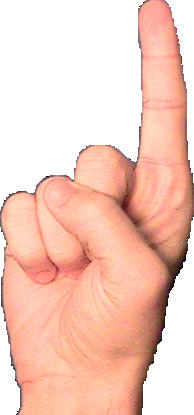
\includegraphics[scale=0.1]{images/01-01-1.jpg}&
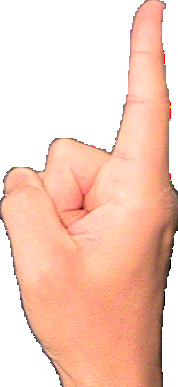
\includegraphics[scale=0.1]{images/01-01-2.jpg}&
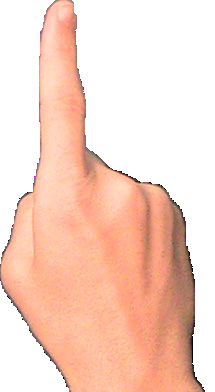
\includegraphics[scale=0.1]{images/01-01-3.jpg}&
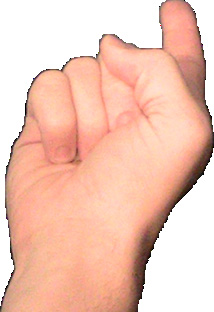
\includegraphics[scale=0.1]{images/01-01-4.jpg}&
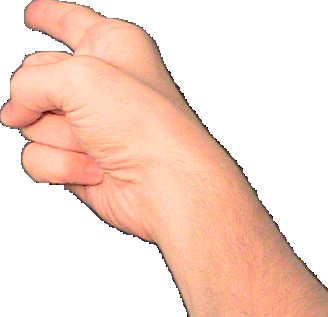
\includegraphics[scale=0.1]{images/01-01-5.jpg}&
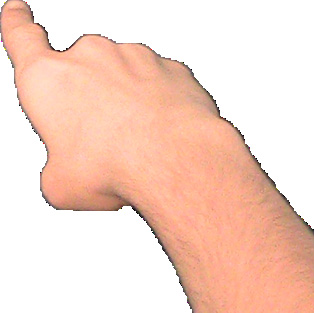
\includegraphics[scale=0.1]{images/01-01-6.jpg}\\
\textbf{Left Hand}&
B508x515S10008493x485&
B508x515S10018493x485&
B508x515S10028493x485&
B508x515S10038493x485&
B508x515S10048493x485&
B508x515S10058493x485\\
\end{tabular}
\end{center}

\subsubsection{The Index on Circle Handshape}

\begin{center}
\begin{tabular}{r*{6}{c}}
&\textbf{Fill 1}&\textbf{Fill 2}&\textbf{Fill 3}&\textbf{Fill 4}&\textbf{Fill 5}&\textbf{Fill 6}\\
\multirow{3}{*}{\textbf{Right Hand}}&
B508x515S10100493x485&
B508x515S10110493x485&
B508x515S10120493x485&
B508x515S10130493x485&
B508x515S10140493x485&
B508x515S10150493x485\\
&
\tikz{\draw[thick](5pt,5pt)circle(5pt);\draw[thick](10pt,20pt)--(10pt,5pt);}&
\tikz{\draw[thick](5pt,5pt)circle(5pt);\draw[thick](10pt,20pt)--(10pt,5pt);\draw[thick](5pt,10pt)--(5pt,0);\draw[thick](8pt,2pt)--(5pt,10pt);\draw[thick](8pt,8pt)--(5pt,0);}&
\tikz{\draw[thick](5pt,5pt)circle(5pt);\draw[thick](0,20pt)--(0,5pt);\draw[thick](2pt,2pt)--(8pt,8pt);\draw[thick](2pt,8pt)--(8pt,2pt);}&
\tikz{\draw[thick](5pt,5pt)circle(5pt);\draw[thick](10pt,20pt)--(10pt,5pt);\draw[thick](5pt,15pt)--(13pt,15pt);}&
\tikz{\draw[thick](5pt,5pt)circle(5pt);\draw[thick](10pt,20pt)--(10pt,5pt);\draw[thick](5pt,10pt)--(5pt,0);\draw[thick](8pt,2pt)--(5pt,10pt);\draw[thick](8pt,8pt)--(5pt,0);\draw[thick](5pt,15pt)--(13pt,15pt);}&
\tikz{\draw[thick](5pt,5pt)circle(5pt);\draw[thick](0,20pt)--(0,5pt);\draw[thick](2pt,2pt)--(8pt,8pt);\draw[thick](2pt,8pt)--(8pt,2pt);\draw[thick](-3pt,15pt)--(5pt,15pt);}\\
&
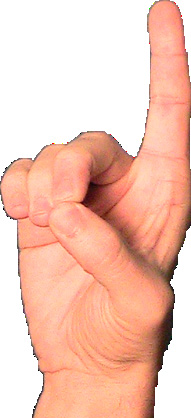
\includegraphics[scale=0.1]{images/01-02-1.jpg}&
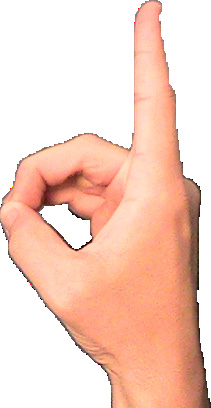
\includegraphics[scale=0.1]{images/01-02-2.jpg}&
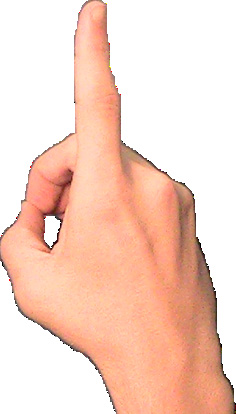
\includegraphics[scale=0.1]{images/01-02-3.jpg}&
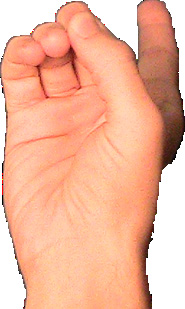
\includegraphics[scale=0.1]{images/01-02-4.jpg}&
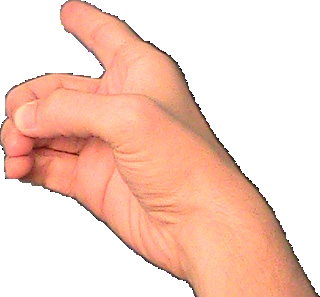
\includegraphics[scale=0.1]{images/01-02-5.jpg}&
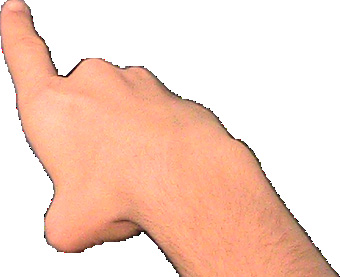
\includegraphics[scale=0.1]{images/01-02-6.jpg}\\
\textbf{Left Hand}&
B508x515S10108493x485&
B508x515S10118493x485&
B508x515S10128493x485&
B508x515S10138493x485&
B508x515S10148493x485&
B508x515S10158493x485\\
\end{tabular}
\end{center}

As you practice to write these don't forget to practice rotations as well!

\subsubsection{The Index on Angle Handshape}

\begin{center}
\begin{tabular}{r*{6}{c}}
&\textbf{Fill 1}&\textbf{Fill 2}&\textbf{Fill 3}&\textbf{Fill 4}&\textbf{Fill 5}&\textbf{Fill 6}\\
\multirow{3}{*}{\textbf{Right Hand}}&
B508x515S10500493x485&
B508x515S10510493x485&
B508x515S10520493x485&
B508x515S10530493x485&
B508x515S10540493x485&
B508x515S10550493x485\\
&
\tikz{\draw[thick](0,0)rectangle(5pt,10pt);\draw[thick](5pt,20pt)--(5pt,0);\draw[thick](-10pt,10pt)--(0,10pt);\draw[thick](0,5pt)--(-7pt,10pt);}&
\tikz{\draw[thick](0,0)rectangle(5pt,10pt);\draw[thick](2.5pt,10pt)--(2.5pt,0);\draw[thick](2.5pt,10pt)--(5pt,0);\draw[thick](5pt,10pt)--(2.5pt,0);\draw[thick](5pt,20pt)--(5pt,0);\draw[thick](-10pt,10pt)--(0,10pt);\draw[thick](0,5pt)--(-7pt,10pt);}&
\tikz{\draw[thick](0,0)rectangle(5pt,10pt);\draw[thick](0,10pt)--(5pt,0);\draw[thick](5pt,10pt)--(0,0);\draw[thick](0,20pt)--(0,0);\draw[thick](-10pt,10pt)--(0,10pt);\draw[thick](0,5pt)--(-7pt,10pt);}&
\tikz{\draw[thick](0,0)rectangle(5pt,10pt);\draw[thick](5pt,20pt)--(5pt,0);\draw[thick](-10pt,10pt)--(0,10pt);\draw[thick](0,5pt)--(-7pt,10pt);\draw[thick](-10pt,5pt)--(10pt,20pt);}&
\tikz{\draw[thick](0,0)rectangle(5pt,10pt);\draw[thick](2.5pt,10pt)--(2.5pt,0);\draw[thick](2.5pt,10pt)--(5pt,0);\draw[thick](5pt,10pt)--(2.5pt,0);\draw[thick](5pt,20pt)--(5pt,0);\draw[thick](-10pt,10pt)--(0,10pt);\draw[thick](0,5pt)--(-7pt,10pt);\draw[thick](-10pt,5pt)--(10pt,20pt);}&
\tikz{\draw[thick](0,0)rectangle(5pt,10pt);\draw[thick](0,10pt)--(5pt,0);\draw[thick](5pt,10pt)--(0,0);\draw[thick](0,20pt)--(0,0);\draw[thick](-10pt,10pt)--(0,10pt);\draw[thick](0,5pt)--(-7pt,10pt);\draw[thick](-10pt,5pt)--(10pt,20pt);}\\
&
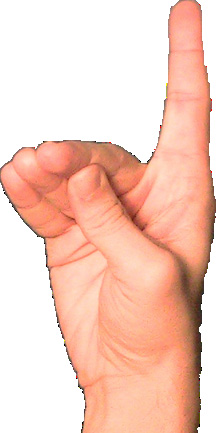
\includegraphics[scale=0.1]{images/01-03-1.jpg}&
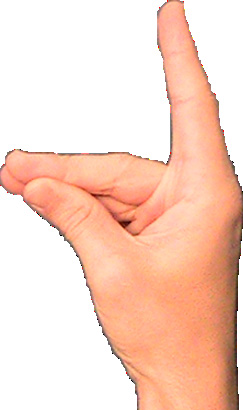
\includegraphics[scale=0.1]{images/01-03-2.jpg}&
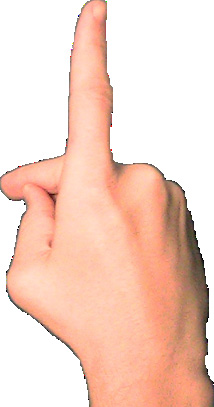
\includegraphics[scale=0.1]{images/01-03-3.jpg}&
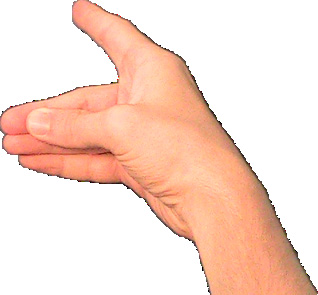
\includegraphics[scale=0.1]{images/01-03-4.jpg}&
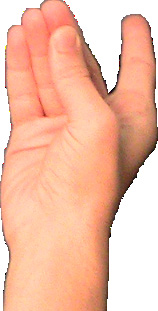
\includegraphics[scale=0.1]{images/01-03-5.jpg}&
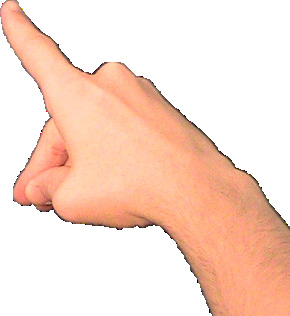
\includegraphics[scale=0.1]{images/01-03-6.jpg}\\
\textbf{Left Hand}&
B508x515S10508493x485&
B508x515S10518493x485&
B508x515S10528493x485&
B508x515S10538493x485&
B508x515S10548493x485&
B508x515S10558493x485\\
\end{tabular}
\end{center}

\subsubsection{The Index Bent Handshape}

\begin{center}
\begin{tabular}{r*{6}{c}}
&\textbf{Fill 1}&\textbf{Fill 2}&\textbf{Fill 3}&\textbf{Fill 4}&\textbf{Fill 5}&\textbf{Fill 6}\\
\multirow{2}{*}{\textbf{Right Hand}}&
B500x500S10600500x500&
B500x500S10610500x500&
B500x500S10620500x500&
B500x500S10630500x500&
B500x500S10640500x500&
B500x500S10650500x500\\
&
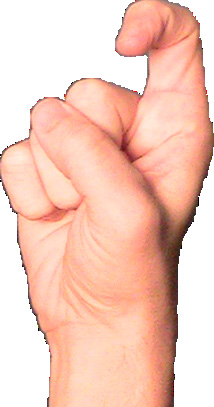
\includegraphics[scale=0.1]{images/01-04-1.jpg}&
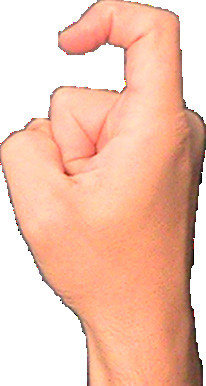
\includegraphics[scale=0.1]{images/01-04-2.jpg}&
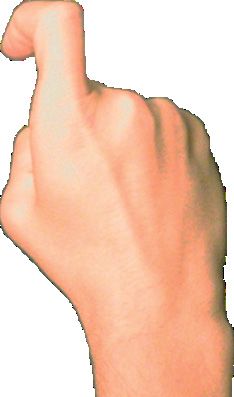
\includegraphics[scale=0.1]{images/01-04-3.jpg}&
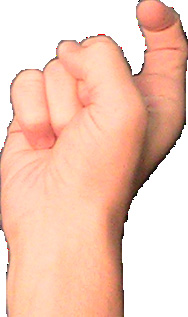
\includegraphics[scale=0.1]{images/01-04-4.jpg}&
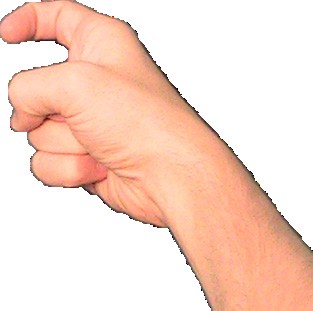
\includegraphics[scale=0.1]{images/01-04-5.jpg}&
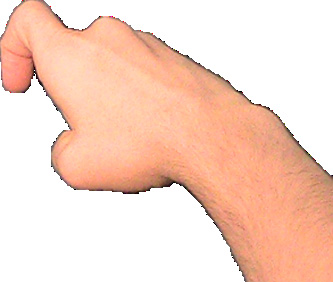
\includegraphics[scale=0.1]{images/01-04-6.jpg}\\
\textbf{Left Hand}&
B500x500S10608500x500&
B500x500S10618500x500&
B500x500S10628500x500&
B500x500S10638500x500&
B500x500S10648500x500&
B500x500S10658500x500\\
\end{tabular}
\end{center}

\subsubsection{The Index Cup Handshape}

\begin{center}
\begin{tabular}{r*{6}{c}}
&\textbf{Fill 1}&\textbf{Fill 2}&\textbf{Fill 3}&\textbf{Fill 4}&\textbf{Fill 5}&\textbf{Fill 6}\\
\multirow{2}{*}{\textbf{Right Hand}}&
B500x500S10a00500x500&
B500x500S10a10500x500&
B500x500S10a20500x500&
B500x500S10a30500x500&
B500x500S10a40500x500&
B500x500S10a50500x500\\
&
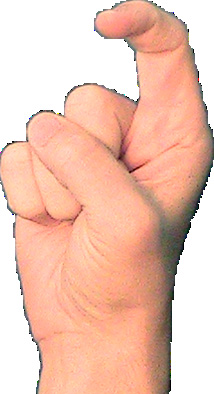
\includegraphics[scale=0.1]{images/01-05-1.jpg}&
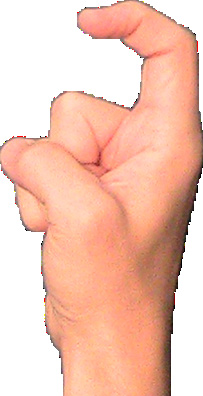
\includegraphics[scale=0.1]{images/01-05-2.jpg}&
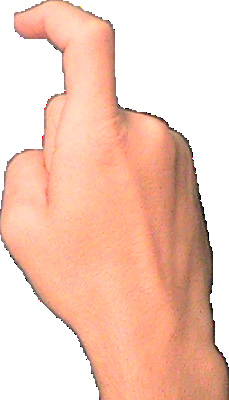
\includegraphics[scale=0.1]{images/01-05-3.jpg}&
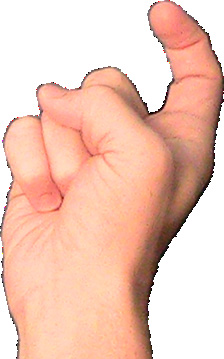
\includegraphics[scale=0.1]{images/01-05-4.jpg}&
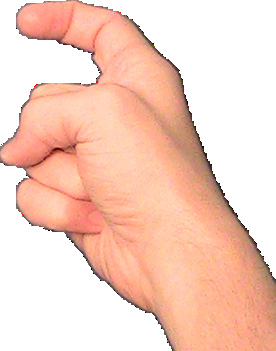
\includegraphics[scale=0.1]{images/01-05-5.jpg}&
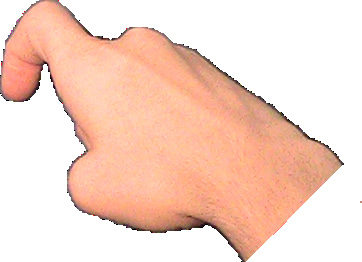
\includegraphics[scale=0.1]{images/01-05-6.jpg}\\
\textbf{Left Hand}&
B500x500S10a08500x500&
B500x500S10a18500x500&
B500x500S10a28500x500&
B500x500S10a38500x500&
B500x500S10a48500x500&
B500x500S10a58500x500\\
\end{tabular}
\end{center}

\subsection{Vocabulary}

\begin{glossary}

\textbf{6}\\
AS18720M509x515S18720491x486

\textbf{7}\\
AS1a520M511x514S1a520490x486

\textbf{8}\\
AS1bb20M511x514S1bb20490x486

\textbf{9}\\
AS1ce20M511x515S1ce20489x485

\textbf{10}\\
AS1f540S2a538M512x528S1f540489x504S2a538493x473

\textbf{a (letter)}\\
AS1f720M510x508S1f720490x493

\textbf{address}\\
AS1f502S1f50aS22a20M520x522S1f502505x498S1f50a480x498S22a20493x478

\textbf{alone}\\
AS10000S2e806M516x525S10000492x495S2e806484x475

\textbf{b}\\
AS14720M507x511S14720493x489

\textbf{boy}\\
AS18510S26500S22104S2ff00M545x522S26500524x507S18510520x489S22104527x476S2ff00482x483

\textbf{brother}\\
AS1dc51S1dc42S1dc4aS20500S22b03S2ff00M538x568S1dc51508x466S1dc4a490x544S1dc42464x526S20500475x553S22b03501x512S2ff00482x483

\textbf{c}\\
AS16d20M509x510S16d20492x490

\textbf{child}\\
AS15a50S22f04M513x524S15a50494x476S22f04488x510

\textbf{children}\\
AS15a50S22a04S2d508M522x525S15a50478x475S22a04483x510S2d508500x511

\textbf{d}\\
AS10110M508x515S10110492x485

\textbf{dad}\\
AS14c10S20500S2ff00M518x518S2ff00482x483S20500495x469S14c10468x453

\textbf{divorce}\\
AS10140S10148S28905S20500S2891dS2fb04M535x531S10140504x469S10148484x469S20500498x473S28905508x504S2891d466x504S2fb04494x525

\textbf{e}\\
AS14a20M508x508S14a20493x493

\textbf{f}\\
AS1ce20M511x515S1ce20489x485

\textbf{fingerspell}\\
AS14c50S26606S22520M529x523S14c50476x492S22520472x478S26606499x505

\textbf{g}\\
AS1f000M515x508S1f000486x493

\textbf{girl}\\
AS1f540S22a03S20e00S2ff00M525x554S1f540510x509S22a03486x540S20e00497x531S2ff00482x483

\textbf{grandma}\\
AS14c10S20500S2b901S2ff00M535x539S2ff00482x483S14c10473x508S2b901509x506S20500497x519

\textbf{grandpa}\\
AS14c10S20500S2b901S2ff00M535x518S2ff00482x483S14c10468x454S2b901509x457S20500496x468

\textbf{h}\\
AS11502M515x508S11502485x493

\textbf{have}\\
AS18041S18049S20500S20500M532x518S18049468x483S18041507x483S20500486x507S20500504x507

\textbf{hey}\\
AS14c50S23504M519x528S14c50490x472S23504482x510

\textbf{how}\\
AS16740S16748S20500S2c400M538x524S20500484x491S2c400498x501S16740491x477S16748462x477

\textbf{how many}\\
AS20330S20330S22a20S14c00S14c08M526x535S22a20494x501S14c08474x465S14c00503x465S20338478x520S20330508x520

\textbf{husband}\\
AS16d10S22b03S16d51S16d09S20800S2ff00M537x564S16d03474x544S16d51489x526S16d10520x483S2ff00482x483S22b03510x506S20800494x553

\textbf{i (letter)}\\
AS19220M511x510S19220490x491

\textbf{j}\\
AS19220S2a20cM519x519S19220498x500S2a20c481x482

\textbf{just}\\
AS10020S2ed09M512x522S2ed09493x479S10020489x492

\textbf{k}\\
AS14020M515x515S14020486x485

\textbf{l}\\
AS1dc20M512x515S1dc20488x485

\textbf{lady}\\
AS1f540S20e00S22a03S14c10S20f00S2c400S2ff00M546x582S22a03502x526S20e00513x513S14c10483x551S2ff00482x483S20f00514x567S1f540527x502S2c400506x541

\textbf{life}\\
AS1f502S1f50aS22a20M520x522S1f502505x498S1f50a480x498S22a20493x478

\textbf{live}\\
AS1f502S1f50aS22a20M520x522S1f502505x498S1f50a480x498S22a20493x478

\textbf{m}\\
AS18d20M510x513S18d20490x488

\textbf{male}\\
AS18510S26500S22104S2ff00M545x522S26500524x507S18510520x489S22104527x476S2ff00482x483

\textbf{man}\\
AS14c10S20500S22c04S20500S2ff00M518x549S2ff00482x483S22c04493x494S14c10467x459S20500495x470S20500495x538

\textbf{many}\\
AS20300S20300S22a24S14c30S14c38M531x536S20300475x464S20300513x464S14c30507x505S14c38470x505S22a24495x486

\textbf{marriage}\\
AS17107S16d21S22b03M528x528S22b03504x472S17107478x502S16d21472x508

\textbf{marry}\\
AS17107S16d21S22b03M528x528S22b03504x472S17107478x502S16d21472x508

\textbf{married}\\
AS17107S16d21S22b03M528x528S22b03504x472S17107478x502S16d21472x508

\textbf{mom}\\
AS14c10S20500S2ff00M518x535S2ff00482x483S20500494x520S14c10471x504

\textbf{n}\\
AS11920M511x513S11920490x487

\textbf{o}\\
AS17620M508x508S17620492x492

\textbf{only}\\
AS10020S2ed09M512x522S2ed09493x479S10020489x492

\textbf{p}\\
AS14021M516x512S14021485x488

\textbf{parents}\\
AS14c10S20500S20500S14c10S22a00S2ff00M518x541S2ff00482x483S14c10466x457S14c10465x510S20500494x471S20500494x519S22a00466x492

\textbf{q}\\
AS1f021M515x512S1f021485x489

\textbf{r}\\
AS11a20M508x515S11a20493x485

\textbf{s}\\
AS20320M508x508S20320493x493

\textbf{single}\\
AS10000S2e806M516x525S10000492x495S2e806484x475

\textbf{sister}\\
AS1dc50S22a03S1dc0aS1dc02S20500S2ff00M539x571S2ff00482x483S1dc50515x494S1dc0a500x547S1dc02474x530S20500487x557S22a03509x524

\textbf{someone}\\
AS10000S2e806M516x525S10000492x495S2e806484x475

\textbf{something}\\
AS10000S2e806M516x525S10000492x495S2e806484x475

\textbf{spell}\\
AS14c50S26606S22520M529x523S14c50476x492S22520472x478S26606499x505

\textbf{t}\\
AS1fb20M508x510S1fb20493x491

\textbf{u}\\
AS11520M508x515S11520493x485

\textbf{v}\\
AS10e20M508x515S10e20493x485

\textbf{w}\\
AS18720M509x515S18720491x486

\textbf{wife}\\
AS16d10S22a03S16d51S16d39S20800S2ff00M527x581S2ff00482x483S22a03506x535S16d51486x546S16d10510x513S20800498x568S16d39470x561

\textbf{woman}\\
AS14c27S22a04S14c10S20500S2ff00M530x583S2ff00482x483S14c27504x508S14c10486x552S20500512x563S22a04495x534

\textbf{work}\\
AS20350S2035aS20600M521x516S20350480x485S2035a490x501S20600499x486

\textbf{x}\\
AS10620M511x513S10620490x487

\textbf{y}\\
AS19a20M514x510S19a20486x490

\textbf{z}\\
AS10020S2450aM519x518S10020481x488S2450a488x483

\end{glossary}

\subsection{Practice Sheet 2.A}

\begin{multicols}{5}
\begin{center}

M508x515S10000493x485 % 1
M536x504S38800464x496 % .
M519x528S14c50490x472S23504482x510 % hey
M537x504S38700463x496 % ,
M510x523S10040495x493S26500491x478 % you
M518x518S30c00482x483 % \?
M522x525S11541498x491S11549479x498S20600489x476 % name
M536x507S38900464x493 % ?
\vfil
\columnbreak

M508x515S10e00493x485 % 2
M536x504S38800464x496 % .
M528x528S22b03504x472S17107478x502S16d21472x508 % marry
M518x518S30a00482x483 % y/n
M510x523S10040495x493S26500491x478 % you
M536x507S38900464x493 % ?
\vfil
\columnbreak

M512x515S11e00489x485 % 3
M536x504S38800464x496 % .
M518x518S30a00482x483 % y/n
M522x525S15a50478x475S22a04483x510S2d508500x511 % children
M510x523S10040495x493S26500491x478 % you
M536x507S38900464x493 % ?
\vfil
\columnbreak

M511x516S14400489x485 % 4
M536x504S38800464x496 % .
M539x571S2ff00482x483S1dc50515x494S1dc0a500x547S1dc02474x530S20500487x557S22a03509x524 % sister
M510x523S10040495x493S26500491x478 % you
M518x518S30c00482x483 % \?
M526x535S22a20494x501S14c08474x465S14c00503x465S20338478x520S20330508x520 % how many
M536x507S38900464x493 % ?
\vfil
\columnbreak

M512x516S14c00489x485 % 5
M536x504S38800464x496 % .
M507x523S15a28494x496S26500493x477 % your
M518x535S2ff00482x483S20500494x520S14c10471x504 % mom
M518x518S30c00482x483 % \?
M522x525S11541498x491S11549479x498S20600489x476 % name
M536x507S38900464x493 % ?
\vfil

\end{center}
\end{multicols}

\subsection{Practice Sheet 2.B}

\begin{multicols}{5}
\begin{center}
M509x515S18720491x486 % 6
M536x504S38800464x496 % .
M518x518S30a00482x483 % y/n
M507x523S15a28494x496S26500493x477 % your
M518x518S2ff00482x483S20500495x469S14c10468x453 % dad
M544x531S20500509x515S10011523x501S20500520x488S2ff00482x483 % deaf
M536x507S38900464x493 % ?
\vfil
\columnbreak

M511x514S1a520490x486 % 7
M536x504S38800464x496 % .
M510x523S10040495x493S26500491x478 % you
M521x516S20350480x485S2035a490x501S20600499x486 % work
M518x518S30c00482x483 % \?
M518x525S10020482x476S27106503x485 % where
M536x507S38900464x493 % ?
\vfil
\columnbreak

M511x514S1bb20490x486 % 8
M536x504S38800464x496 % .
M510x523S10040495x493S26500491x478 % you
M520x522S1f502505x498S1f50a480x498S22a20493x478 % live
M518x518S30c00482x483 % \?
M518x525S10020482x476S27106503x485 % where
M536x507S38900464x493 % ?
\vfil
\columnbreak

M511x515S1ce20489x485 % 9
M536x504S38800464x496 % .
M515x519S10047485x498S26507501x481 % 3rd person
M518x518S30a00482x483 % y/n
M513x520S15a20487x493S26507500x481 % his / hers / its
M536x507S38900464x493 % ?
\vfil
\columnbreak

M513x528S2a538494x472S1f540488x504 % 10
M536x504S38800464x496 % .
M509x515S18720491x486 % w
M508x508S14a20493x493 % e
M518x518S30c00482x483 % \?
M523x535S2ea48483x510S10011502x466S2ea04508x500S10019477x475 % sign (as in ``signing'')
M536x507S38900464x493 % ?
\vfil

\end{center}
\end{multicols}

\subsection{Practice Sheet 2.C}

\begin{multicols}{5}
\begin{center}
M512x520S10000489x490S21d00494x480 % 11
M536x504S38800464x496 % .
M510x523S10040495x493S26500491x478 % you
M522x525S11541498x491S11549479x498S20600489x476 % name
B507x511S14720493x489 % b
B508x508S17620492x492 % o
B507x511S14720493x489 % b
M537x504S38700463x496 % ,
M518x518S30a00482x483 % y/n
M510x523S10040495x493S26500491x478 % you
M536x507S38900464x493 % ?
\vfil
\columnbreak

M509x521S10e00491x491S21d00491x480 % 12
M536x504S38800464x496 % .
M510x523S10040495x493S26500491x478 % you
M535x531S10140504x469S10148484x469S20500498x473S28905508x504S2891d466x504S2fb04494x525 % divorce
M518x518S30a00482x483 % y/n
M510x523S10040495x493S26500491x478 % you
M536x507S38900464x493 % ?
\vfil
\columnbreak

M513x519S22114487x481S12d00489x489 % 13
M536x504S38800464x496 % .
M538x568S1dc51508x466S1dc4a490x544S1dc42464x526S20500475x553S22b03501x512S2ff00482x483 % brother
M510x523S10040495x493S26500491x478 % you
M518x518S30c00482x483 % \?
M526x535S22a20494x501S14c08474x465S14c00503x465S20338478x520S20330508x520 % how many
M536x507S38900464x493 % ?
\vfil
\columnbreak

M513x515S14700493x493S22114487x486 % 14
M536x504S38800464x496 % .
M518x518S30a00482x483 % y/n
M510x523S10040495x493S26500491x478 % you
M532x518S18049468x483S18041507x483S20500486x507S20500504x507 % have
M539x571S2ff00482x483S1dc50515x494S1dc0a500x547S1dc02474x530S20500487x557S22a03509x524 % sister
M536x507S38900464x493 % ?
\vfil
\columnbreak

M513x518S22114487x483S15d00494x491 % 15
M536x504S38800464x496 % .
M507x523S15a28494x496S26500493x477 % your
M518x518S2ff00482x483S20500495x469S14c10468x453 % dad
M522x525S11541498x491S11549479x498S20600489x476 % name
M537x504S38700463x496 % ,
M518x518S30c00482x483 % \?
M529x523S14c50476x492S22520472x478S26606499x505 % fingerspell
M523x524S26503497x511S21100490x497S15a57477x476S15a51500x481
M536x504S38800464x496 % .
\vfil

\end{center}
\end{multicols}

\subsection{Practice Sheet 2.D}

\begin{multicols}{5}
\begin{center}
M520x522S18700502x492S2e00e480x479 % 16
M536x504S38800464x496 % .
M514x536S10008487x464S10020493x471S20500505x469S26600492x506 % you meet
M513x514S15a01490x486S20500487x503 % my
M538x568S1dc51508x466S1dc4a490x544S1dc42464x526S20500475x553S22b03501x512S2ff00482x483 % brother
M518x518S30a00482x483 % y/n
M510x523S10040495x493S26500491x478 % you
M536x507S38900464x493 % ?
\vfil
\columnbreak

M522x522S1a500501x494S2e00e478x478 % 17
M536x504S38800464x496 % .
M507x523S15a28494x496S26500493x477 % your
M527x581S2ff00482x483S22a03506x535S16d51486x546S16d10510x513S20800498x568S16d39470x561 % wife
M518x518S30c00482x483 % \?
M522x525S11541498x491S11549479x498S20600489x476 % name
M536x507S38900464x493 % ?
\vfil
\columnbreak

M523x522S1bb00502x492S2e00e478x479 % 18
M536x504S38800464x496 % .
M507x523S15a28494x496S26500493x477 % your
M539x571S2ff00482x483S1dc50515x494S1dc0a500x547S1dc02474x530S20500487x557S22a03509x524 % sister
M518x518S30a00482x483 % y/n
M516x525S10000492x495S2e806484x475 % single
M536x507S38900464x493 % ?
\vfil
\columnbreak

M524x522S1ce00502x490S2e00e477x479 % 19
M536x504S38800464x496 % .
M535x539S2ff00482x483S14c10473x508S2b901509x506S20500497x519 % grandma
M518x518S30c00482x483 % \?
M522x525S11541498x491S11549479x498S20600489x476 % name
M536x507S38900464x493 % ?
\vfil
\columnbreak

M517x513S22114484x488S1f420488x498 % 20
M536x504S38800464x496 % .
M508x510S1fb20493x491 % t
M515x508S11502485x493 % h
M508x508S14a20493x493 % e
M514x510S19a20486x490 % y
M518x518S30c00482x483 % \?
M523x535S2ea48483x510S10011502x466S2ea04508x500S10019477x475 % sign (as in ``signing'')
M536x507S38900464x493 % ?
\end{center}
\end{multicols}

\subsection{Story 2.A}

\begin{multicols}{5}
\begin{center}
M547x518S2ff00482x483S22a07534x476S14711519x487 % hi
M536x504S38800464x496 % .

M518x518S10043488x483S20500482x507 % me
M507x511S14720493x489 % b
M511x510S19220490x491 % i
M512x515S1dc20488x485 % l
M512x515S1dc20488x485 % l
M537x504S38700463x496 % ,
M508x515S10e20493x485 % v
M511x510S19220490x491 % i
M509x510S16d20492x490 % c
M510x508S1f720490x493 % a
M508x515S11a20493x485 % r
M508x508S20320493x493 % s
M537x504S38700463x496 % ,
M536x511S38a00464x490 % :
M536x511S38a00464x490 % :
M536x504S38800464x496 % .

M544x531S20500509x515S10011523x501S20500520x488S2ff00482x483 % deaf
M518x518S10043488x483S20500482x507 % me
M536x504S38800464x496 % .

M528x560S22a03497x526S17107479x534S16d21473x540S17107512x511S2ff00482x483 % wife
M507x511S14720493x489 % b
M508x508S14a20493x493 % e
M512x515S1dc20488x485 % l
M511x510S19220490x491 % i
M511x513S11920490x487 % n
M508x515S10110492x485 % d
M510x508S1f720490x493 % a
M537x504S38700463x496 % ,
M515x519S10047485x498S26507501x481 % she
M544x531S20500509x515S10011523x501S20500520x488S2ff00482x483 % deaf
M536x504S38800464x496 % .

M511x516S14400489x485 % 4
M522x525S15a50478x475S22a04483x510S2d508500x511 % children
M537x504S38700463x496 % ,
M518x540S14408493x509S10003487x460S20500483x498S20500495x493S20500508x499S2d508489x483 % first three of four
M532x549S2ff00482x483S2ea08495x524S10012502x510 % hearing
M533x525S14408467x494S10003503x476S20500492x497 % last one of four
M544x531S20500509x515S10011523x501S20500520x488S2ff00482x483 % deaf
M518x523S30300482x477 % nod
M533x525S14408467x494S10003503x476S20500492x497 % last one of four
M537x504S38700463x496 % ,
M508x515S10e00493x485 % 2
M545x522S26500524x507S18510520x489S22104527x476S2ff00482x483 % boy
M518x540S14408493x509S10003487x460S20500483x498S20500508x499S2d508489x483 % first and third of four
M525x554S1f540510x509S22a03486x540S20e00497x531S2ff00482x483 % girl
M521x537S14408479x506S10003491x464S20500482x492S20500504x505S2d509495x489 % second and fourth of four
M537x504S38700463x496 % ,
M517x531S14408491x500S10003487x469S20500484x492 % first of four
M512x515S1dc20488x485 % l
M508x508S17620492x492 % o
M515x508S1f000486x493 % g
M510x508S1f720490x493 % a
M511x513S11920490x487 % n
M537x504S38700463x496 % ,
M518x534S14408482x503S10003488x467S20500485x490 % second of four
M515x515S14020486x485 % k
M508x508S14a20493x493 % e
M512x515S1dc20488x485 % l
M508x508S20320493x493 % s
M508x508S14a20493x493 % e
M514x510S19a20486x490 % y
M537x504S38700463x496 % ,
M522x532S14408478x501S10003492x468S20500488x491 % third of four
M507x511S14720493x489 % b
M508x508S14a20493x493 % e
M511x513S11920490x487 % n
M537x504S38700463x496 % ,
M529x527S14408471x496S10003499x474S20500493x496 % fourth of four
M508x508S20320493x493 % s
M510x508S1f720490x493 % a
M508x515S11a20493x485 % r
M510x508S1f720490x493 % a
M515x508S11502485x493 % h
M536x504S38800464x496 % .
\end{center}
\end{multicols}

\subsection{Story 2.B}

\begin{multicols}{5}
\begin{center}
M547x518S2ff00482x483S22a07534x476S14711519x487 % hi
M536x504S38800464x496 % .

M518x518S10043488x483S20500482x507 % me
M515x515S14020486x485 % k
M508x508S14a20493x493 % e
M512x515S1dc20488x485 % l
M508x508S20320493x493 % s
M508x508S14a20493x493 % e
M514x510S19a20486x490 % y
M537x504S38700463x496 % ,
M508x515S10e20493x485 % v
M511x510S19220490x491 % i
M509x510S16d20492x490 % c
M510x508S1f720490x493 % a
M508x515S11a20493x485 % r
M508x508S20320493x493 % s
M536x504S38800464x496 % .

M532x549S2ff00482x483S2ea08495x524S10012502x510 % hearing
M518x518S10043488x483S20500482x507 % me
M536x504S38800464x496 % .

M518x535S2ff00482x483S20500494x520S14c10471x504 % mother
M518x518S2ff00482x483S20500495x469S14c10468x453 % father
M544x531S20500509x515S10011523x501S20500520x488S2ff00482x483 % deaf
M536x504S38800464x496 % .

M518x518S2ff00482x483S20500495x469S14c10468x453 % father
M522x525S11541498x491S11549479x498S20600489x476 % name
M507x511S14720493x489 % b
M511x510S19220490x491 % i
M512x515S1dc20488x485 % l
M512x515S1dc20488x485 % l
M536x504S38800464x496 % .

M518x535S2ff00482x483S20500494x520S14c10471x504 % mother
M507x511S14720493x489 % b
M508x508S14a20493x493 % e
M512x515S1dc20488x485 % l
M511x510S19220490x491 % i
M511x513S11920490x487 % n
M508x515S10110492x485 % d
M510x508S1f720490x493 % a
M536x504S38800464x496 % .

M532x518S18049468x483S18041507x483S20500486x507S20500504x507 % have
M508x515S10e00493x485 % 2
M538x568S1dc51508x466S1dc4a490x544S1dc42464x526S20500475x553S22b03501x512S2ff00482x483 % brother
M508x515S10000493x485 % 1
M539x571S2ff00482x483S1dc50515x494S1dc0a500x547S1dc02474x530S20500487x557S22a03509x524 % siste
M536x504S38800464x496 % .

M517x531S14408491x500S10003487x469S20500484x492 % first of four
M538x568S1dc51508x466S1dc4a490x544S1dc42464x526S20500475x553S22b03501x512S2ff00482x483 % brother
M537x504S38700463x496 % ,
M512x515S1dc20488x485 % l
M508x508S17620492x492 % o
M515x508S1f000486x493 % g
M510x508S1f720490x493 % a
M511x513S11920490x487 % n
M537x504S38700463x496 % ,
M532x549S2ff00482x483S2ea08495x524S10012502x510 % hearing
M537x504S38700463x496 % ,
M528x528S22b03504x472S17107478x502S16d21472x508 % married
M537x504S38700463x496 % ,
M508x515S10e00493x485 % 2
M522x525S15a50478x475S22a04483x510S2d508500x511 % children
M536x504S38800464x496 % .

M518x534S14408482x503S10003488x467S20500485x490 % second of four
M518x518S10043488x483S20500482x507 % me
M537x504S38700463x496 % ,
M516x525S10000492x495S2e806484x475 % single
M536x504S38800464x496 % .

M522x532S14408478x501S10003492x468S20500488x491 % third of four
M538x568S1dc51508x466S1dc4a490x544S1dc42464x526S20500475x553S22b03501x512S2ff00482x483 % brother
M537x504S38700463x496 % ,
M507x511S14720493x489 % b
M508x508S14a20493x493 % e
M511x513S11920490x487 % n
M537x504S38700463x496 % ,
M535x531S10140504x469S10148484x469S20500498x473S28905508x504S2891d466x504S2fb04494x525 % divorced
M537x504S38700463x496 % ,
M508x521S17610492x505S26500494x479 % 0
M522x525S15a50478x475S22a04483x510S2d508500x511 % children
M536x504S38800464x496

M529x527S14408471x496S10003499x474S20500493x496 % four of four
M539x571S2ff00482x483S1dc50515x494S1dc0a500x547S1dc02474x530S20500487x557S22a03509x524 % sister
M537x504S38700463x496 % ,
M508x508S20320493x493 % s
M510x508S1f720490x493 % a
M508x515S11a20493x485 % r
M510x508S1f720490x493 % a
M515x508S11502485x493 % h
M537x504S38700463x496 % ,
M544x531S20500509x515S10011523x501S20500520x488S2ff00482x483 % deaf
M537x504S38700463x496 % ,
M516x525S10000492x495S2e806484x475 % single
M536x504S38800464x496 % .
\end{center}
\end{multicols}

\end{document}

